\documentclass{article}
\title{Solving Learning Parity with Noise Problem using Generalized LF Algorithm}
\author{Subhrajyoty Roy\\
        Indian Statistical Institute\\
       \emph{Email:} roysubhra98@gmail.com}
\date{\today}

\usepackage{amsmath}
\usepackage{algorithm}
\usepackage[noend]{algpseudocode}
\usepackage[utf8]{inputenc}
\usepackage[english]{babel}
\usepackage{amsthm}
\usepackage{graphicx}

\begin{document}
	\maketitle

\begin{abstract}
	The Learning Parity with Noise (LPN) problem is special case of Learning with Errors (LWE) problem that has recently been studied in the world of cryptography due to its hardness assumptions. It is believed that the LPN problem is `NP-hard' and is resistant to quantum computers. Also, due to its simplicity, it is a good candidate to implement in light-weight devices.
	Till today, the best known algorithm to solve LPN problem is due to Blum, Kalai and Wasserman, called BKW algorithm. However, Levieil and Fouque has provided two improved version of that called LF1 and LF2. In IACR-EUROCRYPT 2016, a general version of LF1 and LF2 is proposed called LF(k) due to Zhang, Jiao and Wang. In this paper, the complexity of LF(k) is deeply analyzed. Finally, a method for solving LPN using Hadamard code (LFHC) has been proposed. A heuristic complexity result is also given for LF-HC. Although LF-HC is not better than subsequent LF(k) in terms of query complexity, it may perform better in terms of memory and time complexity. This gives an incentive to use LF-HC in practical problems.\\
	
	\emph{Keywords:} LPN, BKW, LF1, LF2, Hadamard Code.
	
\end{abstract}

\section{The LPN Problem}

  The Learning Parity with Noise problem is based on a setting between a challenger and an adversary who is trying to get hold of the secret vector $s\in \mathbf{Z}_2^n$ given the oracle access to LPN challenger. On each query, challenger randomly picks a vector of length $n$ namely $v\in \mathbf{Z}_2^n$ and chooses an error bit $e\in \{0,1\}$ according to the probablity distribution $Ber(\tau)$ where $\tau \in (0, \frac{1}{2})$. Then it computes the inner product $$c= \langle v,s\rangle\oplus\ e$$ and sends the pair $(v,c)$ to the adversary. Given access to enough number of queries, adversary has to guess the secret vector $s$.\\
  
  We will say that an adversary $A(t,m,q, \theta)$ solves $LPN_{s,n,\tau}$ problem if $$Pr[A^{LPN_{s,n,\tau}} ()=s]\geq\theta$$ and algorithm runs for time $t$, uses memory $m$ and makes $q$ queries, while $\theta$ is the advantage of the adversary. This version of the LPN problem is called `Search LPN Problem'.\\
  
  Let $D^{LPN}_{s,n,\tau}$ be the corresponding probability distribution of outputs of LPN oracle. Then the decisional version of the problem asks an adversary to distinguish between uniform distribution over $\mathbf{Z}_2^{n+1}$ and $D^{LPN}_{s,n,\tau}$. For the rest of the paper, we define the bias $\delta=1-2\tau$ as a measure of this distinguishablity.
  
  
  \section{Known LPN solving Algorithms}
  \subsection[2.1]{BKW Algorithm}
      The BKW algorithm due to Blum, Kalai and Wasserman has been proposed in 2003.  The algorithm uses two phases  -- a reduction phase and a solving phase as described in detail in the paper\cite{BKW}. The reduction phase applies \emph{XOR} to make some bits of $v$ zero, so that the secret is reduced to fewer bits. Finally, in the solving phase, it looks for queries that has hamming weight 1 and applies a majority rule to guess the corresponding bit of secret vector.\\
      
      For ease of understanding, let us assume $n=ab$ where $b$ is blocklength and $a$ is the number of blocks. After having a sufficient amount of queries, in the reduction step, the query vectors $v$ are divided into equivalence classes according to their last $b$ bits. For each equivalence class, choose a representative vector and replace other vectors residing in same class by \emph{XOR} with it and then discard the representative vector. That would make all of their last $b$ bits $0$. This reduction step is repeated $(a-1)$ times so that only first $b$ bits of each vector may remain nonzero. In the solving phase, from the set of reduced queries, only vectors with hamming weight $1$ are chosen. As most of the errors are set to $0$, by taking a majority rule on $c$ for those $v$ vectors, we get the corresponding bit of secret vector $s$.\\
      
      In \cite{LF}, it is shown that BKW solves $LPN_{s,n,\tau}$ problem with $q=20 \ln(4n)2^b\delta^{-2^a} + (a-1)2^b$ queries, in time $t=O(naq)$ using memory $m=nq$ with an advantage of $\theta=\frac{1}{2}$.
      
      \subsection[2.2]{LF1 Algorithm}
      Levieil and Fouque improved the BKW algorithm with the idea that in BKW solving phase, a lot of queries are not being used as they are not of hamming weight $1$. So, they kept the reduction phase as it is, rather introduced a different solving phase using Walsh Hadamard Transformation \cite{LF}. Let us assume $(v',c')$ be a reduced query. Consider the following function:
       $$f(x)=\sum_{v'}\mathbf{1}_{v'=x}(-1)^{c'}$$
        The above function is like a net counting of voting to determine which is the true $c'$  in the whole group where the queries $v'$ are same. Applying Walsh Hadamard transformation on this function for each $b$ length vector $u$, $$\hat{f}(u)=\sum_{x\in\mathbf{Z}_2^{b}}(-1)^{\langle u,x\rangle}f(x)$$ which turns out to be $q-(a-1)2^b- 2HW(V'u^T\oplus\ C')$, where $V'$ is the matrix formed by all reduced query vectors $v'$. For $u=s$, it turns out to be $q-(a-1)2^b-2HW(E')$ and as most of the error vectors are set to $0$, we assume correct guess of $s$ maximizes the value of this transformed function. In \cite{LF} rather than applying naive Walsh Hadamard transformation, a fast Walsh Hadamard transformation is applied to reduce complexity.\\
        
        Given $LPN_{s,n,\tau}$ instance, LF1 with $q=(8b+200)\delta^{-2^a}+(a-1)2^b$, $t= O(naq+b2^b)$, $m=O(nq+b2^b)$ and $\theta=\frac{1}{2}$ solves the problem.
        
    \subsection[2.3]{LF2 Algorithm}
    The LF2 algorithm as proposed in \cite{LF}, is about changing the reduction step of LF1, but preserving the solution step of LF1 as it is. In the reduction step of this algorithm, rather than discarding the representative vector from each class, the algorithm computes all possible pairs in same equivalence class so that \emph{XOR}ing them would get last $b$ bits $0$. Also, there is a chance that the number of queries in each such reduction step grows exponentially faster which may affect the time and memory complexity. To keep them in check as well, the algorithm starts with $3.2^b$ queries because of the identity $\binom{3}{2}=3$ and presence of atmost $2^b$ equivalence classes.\\
    
    The complexity theorem of LF2 shows that it heuristically solves $LPN_{s,n,\tau}$ problem with $q=3.2^b$ queries, in time $t=O(naq+b2^b)$ using memory $m=O(nq+b2^b)$ with advantage $\theta$ satisfying $q=3.2^b\ge 8\ln(\frac{2^b}{\theta})\delta^{-2^a}$.

   \section{Generalized LF Algorithm: LF(k)}
   LF(k) is a generalized Levieil-Fouque algorithm first proposed in \cite{LFk} with parameter $k$ where the solving step remains same as LF1 and LF2 i.e. using a fast Walsh Hadamard transformation. The reduction step concerns about finding sufficient $k$ tuples that \emph{XOR} to $0$ using generalized birthday problem discussed in \cite{Ksum} to solve this $k$-sum problem. The whole algorithm for LF(k) has been discussed in algorithm \ref{LFkalgo}.
   
   \begin{algorithm}
   	\caption{LF(k)} \label{LFkalgo}
   	\begin{algorithmic}[1]
   		\State \emph{Parameters}: $a$, $b$
   		\State \emph{Input}:
   		A set $V$ of $q$ queries $(v_i,c_i)\quad\forall i\in {1,2,...,q}$, where $v_i$s are of length $n$.
   		\State Find sufficient $k$ tuples that add to $0$ in last $b$ bits of $v_i$. Put each such \emph{XOR}-ed results in set $U$ leaving the last $b$ bits of $v_i$ which are already $0$. 
   		\State Accordingly calculate \emph{XOR} of $c_i$s and bind them together with $v_i$s in $U$.
   		\State $V=U$.
   		\State Repeat the above steps $a$ times.
   		\State Now, the size of the secret becomes $n'=n-ab$. 
   		\State Define the function that tracks the net majority count in each group, that is $f(x)=\sum_{(v',c')\in V}\mathbf{1}_{v'=x}(-1)^{c'}$
   		\State Compute Fast Walsh Hadamard transformation of the function $\hat{f}(u)=\sum_{x\in\mathbf{Z}_2^{n'}}(-1)^{\langle u,x\rangle}f(x)$ for every $n'$ length vector $u$.
   		\State $(s_1,s_2,s_3,...,s_{n'})=\arg\max{\hat{f}(u)}$
   	\end{algorithmic}
   \end{algorithm}

  \newtheorem{lemma}{Lemma}
  \newtheorem{theorem}{Theorem}
  
  \subsection[3.1]{Complexity Results of LF(k)}
  The complexity results of LF(k) resembles LF1 and LF2 in a very much way. However, as we will see, the parameter $a$ and $b$ that minimizes the query and time complexity will depend on $k$. To give a rough idea, as we are \emph{XOR}-ing $k$ vectors at a time in the reduction phase, the bias $\delta$ would decrease exponentially making it harder to apply solving phase. So, we need a bigger blocklength $b$ so that the number of reduction steps $a$ remains small. Certainly, that would put a bound on $k$ as the blocklength $b$ should not be too big to handle.
  \begin{lemma}
  	If after \textbf{a} steps of reduction, the amount of query left is $\mathbf{q'}$ and the reduced bias is $\delta'$, then $q'\ge 8\ln(\frac{2^{n'}}{1-\theta})\delta^{'-2}$ should happen to ensure that the adversary suceeds with advantage $\theta$.
  \end{lemma}
  
  \begin{proof}
  	 The prrof of this lemma follows a technique shown in \cite{LPNjournal}. We will try to estimate the failure probability of the algorithm and bound it above by $1-\theta$, as the success probability is bounded below by the advantage $\theta$.\\
  	 
  	 Recall that Walsh transformation yields the function $$\hat{f}(u)=\sum_{x\in\mathbf{Z}_2^{n'}}(-1)^{\langle u,x\rangle}f(x) = \sum_{x\in\mathbf{Z}_2^{n'}}(-1)^{\langle u,x\rangle}\sum_{v'}\mathbf{1}_{v'=x}(-1)^{c'} $$ $$= \sum_{(v',c')\in V}(-1)^{\langle v',u\rangle \oplus c'}=q' - 2HW(V'u^T\oplus C')$$ where $V'$ is the matrix created by writing query vectors $v'$ as rows, and $C'$ is the column vector created from corresponding query answer $c'$. The LF algorithm works on the fact that if $u=s$ then $HW(V's^T\oplus C')=HW(E')$ and as most of the error bits are set to $0$, for correct guess $\hat{f}(u)$ will be maximum.\\
  	 
  	 Therefore, the failure probablity of LF(k) is the probablity of finding a vector $u$ of length $n'$ such that $HW(V'u^T\oplus C')\le HW(V's^T\oplus C')=HW(E')$. Letting, $x=u+s$, we get $HW(V'u^T\oplus C')=HW(V'x^T\oplus E')$. Hence, we obtain that the failure probablity is bounded by $2^{n'}$ times the probability of $HW(V'x^T\oplus E')\le HW(E')$ for a fixed $n'$ bit nonzero vector $x$. Since, $V'$ is uniformly distributed and assuming it to be independent of $E'$, we guess that $V'x^T\oplus E'$ should be unifromly distributed. Call $y=V'x^T\oplus E'$.\\
  	 
  	 We will use Hoeffding's inequality \cite{hoeffding}. Let $X_1, X_2, ..., X_{q'}$ be independent random variables such that $X_i = y_i-e'_i$ which keeps track of difference of their hamming weights. Also, we have $E(y_i-e'_i)=\frac{\delta'}{2}$. Let $X=X_1+X_2+...+X_{q'}$. Taking $\lambda = E[X]=\frac{q'\delta'}{2}$ in the inequality in \cite{hoeffding} to obtain:
  	 
  	 $$Pr[incorrect\quad guess]\leq 2^{n'}Pr[\sum_{i=1}^{q'}(y_i-e'_i)\le 0]\leq 2^{n'}e^{-\frac{q'\delta'^2}{8}}$$
  	 
  	 As the failure probablity is bounded above by $1-\theta$, so equating $1-\theta$ with $2^{n'}e^{-\frac{q'\delta'^2}{8}}$, we get $q'= 8\ln(\frac{2^{n'}}{1-\theta})\delta^{'-2}$, the desired result. 
  \end{proof}
   
   \begin{lemma}
   	The number of initial queries $q$ should approximately  be equal to $(2^b k!)^{{1}/(k-1)}$ so that at any step of reduction the number of queries does not exceed $q$.
   \end{lemma}
 
  \begin{proof}
  	Suppose, $q_i$ be the number of queries at $i$-th step of reduction. Assuming the query vectors are independent and random, their $k$-sum will also be random. Hence, about $2^{-b}$ of all possible vector sums will have $0$ in last $b$ bits. Hence, we expect about $\binom{q_i}{k}2^{-b}$ queries having last $b$ bits equal to $0$ that proceeds to next step of reduction. \\
  	
    We want $q_i\leq q\quad \forall i=1,2,...,a$ and more particularly, we want $\binom{q}{k}2^{-b}\leq q$. Approximating $\binom{q}{k}$ by $\frac{q^k}{k!}$ as $q$ is large, we get $q^{k-1}\leq 2^b k!$ that proves the lemma.
  \end{proof}

  \begin{theorem}\emph{\textbf{[Complexity Theorem of LF(k)]}}
  	Given a $LPN_{s,n,\tau}$ instance with $n=ab+{n'}$, the algorithm LF(k) with $q=(2^bk!)^{{1}/(k-1)}\geq 8\ln(\frac{2^{n'}}{1-\theta})\delta^{-2.k^{a}}$, $t=O(naq+n'2^{n'}+ak(2^bq)^{1/(1+\log_2k)})$, $m=O(nq+n'2^{n'}+k2^{b/(1+\log_2k)})$ heuristically solves the problem with advantage $\theta$.
  \end{theorem}

   \begin{proof}
   	From \emph{Lemma 2} we get that intial number of query $q$ should be equal to $(2^bk!)^{1/(k-1)}$. However, from \emph{Lemma 1}, it follows that the reduced number of queries $q'$ is greater than $8\ln(\frac{2^{n'}}{1-\theta})\delta^{'-2}$, as after $a$ steps of reduction a secret of size $n'$ will remain. Also, Matsui's Piling up Lemma \cite{LF} shows that $\delta'=\delta^{k^{a}}$ as we are \emph{XOR}ing $k$ vectors together at a time. This gives the expression for number of queries.\\
   	For the time and space complexity, the extra cost is solving $k$-sum problem at each step of reduction. In \cite{Ksum}, it has been shown that a single solution of the $k$-sum problem can be found in $k2^{b/(1+\log_2k)}$ time and space, whereas $q$ many solutions can be found in $q^{1/(1+\log_2k)}$ times the work of a single solution. Therefore, this adds a complexity of $k(2^bq)^{1/(1+\log_2k)}$ in time and $k2^{b/(1+\log_2k)}$ in space at each reduction step and we have $O(a)$ such steps. Observe that for memory, we can overwrite the $k$-sum vectors at each reduction step, so it is counted only once. The term $n'2^{n'}$ appears due to implementation of Fast Walsh Hadamard transformation on $2^{n'}$ vectors of length $n'$.\\
   	This proves the complexity result.
   \end{proof}
 
   As the above theorem shows, the extra cost of solving $k$-sum problem is using $2^{b/(1+\log_2k)}$ time and space which can be large if $b$ is large. As the bias reduces exponentially like $\delta^{k^{a}}$, we need $a$ to be small to keep the bias in check. That means $b$ is going to be large and will inflate the time and memory complexity. In \cite{Ksum}, it was stated that the lower bound of computational complexity of $k$-sum problem would be $2^{b/k}$ which implies that LF(k) would perform better if better algorithm for solving $k$-sum problem is known.
 
 \subsection[3.2]{LF-HC (Levieil Fouque Hadamard Code Algorithm)}
 In this section, I will present a variant of LF algorithm that uses Hadamard Code instead of Walsh-Hadamard transformation in solving phase. The idea is closely related to BKW \cite{BKW} majority rule, but it applies the majority rule over all $2^{n'}$ possible reduced query vectors. Then using the $2^{n'}$ vectors each of length $n'$, it constructs the corresponding hadamard code and decode it. As the error correcting code can only decode upto $2^{n'-2}$ errors, so we need the majority rule to be performed to reduce the number of errors.\\
 
 \begin{algorithm}
 	\caption{LF-HC}\label{LFHC}
 	\begin{algorithmic}[1]
 	   \State \emph{Parameters}: $a$, $b$, $k$.
 	   \State Apply LF(k) reduction for suitable $k$ and blocklength $b$.
 	   \State After reduction, the secret is reduced to $n'=n-ab$ bits.
 	   \State Group all reduced queries in $2^{n'}$ equivalence class. In each group, we have a corresponding equation like $\langle v',s\rangle\oplus e'=c'$.
 	   \State Perform a majority rule over each group. As most of the error bits are set to $0$, majority rule gives $\langle v_i',s\rangle=c_i'$ where $c_i'=0$ or $1\quad\forall i=1,2,...,2^{n'}$
 	   \State \emph{For $i \in {1,2,...,n}$:}
 	   \State \qquad Pick $j$ at random from $1,2,...,2^{n'}$
 	   \State \qquad Let $k$ be such that $v_k=v_j\oplus r_i$, where $r_i$ is a vector contianing $1$ at $i$-th position and rest are $0$.
 	   \State \qquad $s_i=c_j\oplus c_k$.
 	\end{algorithmic}
 \end{algorithm}
 
 This algorithm uses reduction phase as LF(k), where it uses a solution phase lying midway between BKW solution (majority rule) and LF solution (Fast Walsh-Hadamard transformation). BKW solution phase uses majority rule to figure out solution to some particular vector queries and that would waste a lot of queries. However, Levieil and Fouque pointed this weakness in \cite{LF} and moved to using Fast Walsh-Hadamard transformation. Here, in algorithm \ref{LFHC} the solution phase uses majority rule to figure out correct solution to every vector queries as shown in \emph{step 4}. However, we may allow about $2^{(n'-2)}=\frac{2^{n'}}{4}$ many errors in majority rule, and use Hadamard code local decoding technique to correct these errors. Heuristically, this will need lesser queries than BKW, while seemingly more queries than LF algorithms. However, with properly chosen parameter this algorithm may perform better than LF1 or LF2, as will be shown in next section.
 
 \subsection[3.3]{Complexity Analysis of LF-HC}
 In this subsection, we will discuss complexity of LF-HC heuristically. If the reduced secret size is $n'$ and number of reduced queries is $q'$, then we expect about $\frac{q'}{2^{n'}}=N$ query vectors in each of the group. Let, $X$ be a random variable that tracks the number of errors in each group. As we apply majority rule, we can allow at most $\frac{1}{4}$-th of groups to get wrong solution to query vectors since Hadamard Code can correct upto $2^{n'-2}$ errors in $2^{n'}$ length codeword, we want $Pr[X\le\frac{N}{2}]\le\frac{1}{4}$.
 
 Also, to use Hoeffding's inquality, we consider the random variables $X_i$ that takes 1 iff $i$-th entry in the group has error, $0$ otherwise. Clearly, $X=X_1 +X_2+...+X_N$ and $Pr[X_i\in[0,1]]=1$. Therefore, we get $$Pr[X\le\frac{N}{2}]=Pr[X\le N\frac{(1-\delta')}{2}+N\frac{\delta'}{2}]\le e^{-2N(\frac{\delta'}{2})^2}$$
 Equating $e^{-2N(\frac{\delta'}{2})^2}$ with $\frac{1}{4}$ we get that $N= 2\ln(4)\delta^{'-2}$. It leads to the number of reduced queries $q'$ to satisfy the relation, $q'\geq 2^{n'}\ln(16)\delta^{-2.k^{a}}$. As the reduced number of queries in LF-HC is same as number of reduced queries in LF(k), the condition for LF-HC to be applied is given by: $$q=(2^bk!)^{1/(k-1)} \geq 2^{n'}\ln(16)\delta^{-2.k^{a}}$$ (first equality follows from \emph{Lemma 2} of Section 3.1).\\
 Hence, the advantage $\theta$ becomes the probabilty of the event that there are less than or equal to $2^{n'-2}$ wrong solution emerged from the majority rule. Therefore, $$\theta=\sum_{i=1}^{2^{n'-2}}\binom{2^{n'}}{i}{(p')}^i{(1-p')^{2^{n'}-i}}$$where $p'$ is the probabilty of getting a wrong solution from majority rule. Therefore, $p'=Pr[X\leq N/2]\leq exp{(-N\delta^{2k^a}/2)}=exp(-\frac{q\delta^{2k^a}}{2^{n'+1}})$.
 
 For time and memory complexity, observe that the Algorithm \ref{LFHC} uses $k$-sum solving, but uses hadamard code decoding using two \emph{XOR}s for each secret bit instead of Fast-Walsh Hadamard transformation. Therefore, in terms of $n'2^{n'}$ term in time and space complexity of LF(k), we would have $n'(n'+1)=O(n'^{2})$ in time and $O(n')$ in space to save the $c_i$'s. Therefore, we get the following theorem:
 
 \begin{theorem}\emph{\textbf{[Complexity Theorem of LF-HC]}}
 	Given $LPN_{s,n,\tau}$ instance, LF-HC algorithm with $q=(2^bk!)^{1/(k-1)} \geq 2^{n'}\ln(16)\delta^{-2.k^{a}}$, $t=O(naq+n'(n'+1)+ak(2^bq)^{1/(1+\log_2k)})$, $m=O(nq+n'+k2^{b/(1+\log_2k)})$ heuristically solves the problem with advantage $$\theta\geq\sum_{i=1}^{2^{n'-2}}\binom{2^{n'}}{i}{(p')}^i{(1-p')^{2^{n'}-i}}$$, where $p'=\emph{exp}{(-\frac{q\delta^{2.k^{a}}}{2^{n'+1}})}$. Particularly, with queries $q\geq 3.2^{n'}\delta^{-2.k^{a}}$ the advantage becomes more than $\frac{1}{2}$.
 \end{theorem}
 
 \section{Comparison of LPN solving Algorithms}
  There are many specific instances of the LPN problem. In this section, BKW, LF1, LF2, LF-HC will be compared in terms of query and time complexity. However, to implement LF(k) and LF-HC, it is better not to take the parameter $k$ to be larger than $4$, as suggested in \cite{LFk} also. In \cite{Ksum}, it is stated that for $k=4$, the extra cost in time and memory complexity will be of order $2^{b/3}$ which should be of almost same order of $O(naq)$ parts. For this reason, LF-HC algorithm mostly uses $k=4$ as the parameter to achieve better results. However, similar to LF(k), if better algorithm to solve $k$-sum problem is known, then it can be used to further improve the algorithms.
 
 
 	\begin{table}
 		\begin{center}
 	\begin{tabular}{|c|c|c|c|c|c|c|}
 		\hline
 		\multicolumn{2}{|c|}{Instance}
 	&	\multicolumn{2}{|c|}{BKW}
 	&	\multicolumn{2}{|c|}{LF1}\\
 	    \hline
 		secret size & $\tau$ & b & query($\log_2q$) & b & query($\log_2q$)\\
 		\hline
 		256 & 0.25 & 64 & 82.79 & 52 & 54\\
 		512 & 0.125 & 86 & 115.49 & 74 & 76.58\\
 		592 & 0.125 & 99 & 128.52 & 85 & 87.59\\
 		768 & 0.05 & 110 & 132.46 & 86 & 89.46\\
 		1024 & 0.01 & 114 & 131.98 & 94 & 97.32\\
 		\hline
 	\end{tabular}
 \\
 	\begin{tabular}{|c|c|c|c|c|c|c|}
 	\hline
 	\multicolumn{2}{|c|}{Instance}
 	&	\multicolumn{2}{|c|}{LF2}
 	&	\multicolumn{2}{|c|}{LF4}\\
 	\hline
 	secret size & $\tau$ & b & query($\log_2q$) & b & query($\log_2q$)\\
 	\hline
 	256 & 0.25 & 52 & 53.58 & 116 & 40.19\\
 	512 & 0.125 & 74 & 75.58 & 170 & 58.19\\
 	592 & 0.125 & 85 & 86.58 & 180 & 61.52\\
 	768 & 0.05 & 86 & 87.58 & 193 & 65.86\\
 	1024 & 0.01 & 94 & 95.58 & 200 & 68.19\\
 	\hline
 \end{tabular}
\\
	\begin{tabular}{|c|c|c|c|}
	\hline
	\multicolumn{2}{|c|}{Instance}
	&	\multicolumn{2}{|c|}{LF-HC}\\
	\hline
	secret size & $\tau$ & b & query($\log_2q$)\\
	\hline
	256 & 0.25 & 124 & 42.86\\
	512 & 0.125 & 170 & 58.19\\
	592 & 0.125 & 194 & 66.19\\
	768 & 0.05 & 237 & 80.53\\
	1024 & 0.01 & 204 & 69.52\\
	\hline
\end{tabular}
  \caption{Query Complexity for different instances of LPN for different algortihms}
  \label{table1}
\end{center}
 \end{table}
 
 
 \begin{table}
 	\begin{center}
 		\begin{tabular}{|c||c|c|c|c|}
 			\hline
 			Algorithm & b & Query ($\log_2q$) & Time ($\log_2t$) & Memory ($\log_2m$)\\
 			\hline
 			BKW & 86 & 115.49 & 127.07 & 124.49\\
 			LF1 & 74 & 76.58 & 88.39 & 85.58\\
 			LF2 & 74 & 75.58 & 87.39 & 84.58\\
 			LF4 & 170 & 58.19 & 78.07 & 67.19\\
 			LF-HC & 170 & 58.19 & 78.07 & 67.19\\
 			\hline 
 		\end{tabular}
 	\caption{Algorithms complexity when used to solve $LPN_{s,512,\frac{1}{8}}$ instance}
 	\label{table2}
 	\end{center}
 \end{table}
 
 As seen from the Table \ref{table1}, LF-HC performs better than BKW, LF1 and LF2. However, as suggested before, these instances use $k=4$ in LF-HC and it is seen to be optimal. Therefore, on certain instances $(LPN_{s,512,0.125})$, it performs almost like LF(4) algorithm, while in certain cases $(LPN_{s,768,0.05})$, it performs worse than LF(4), in terms of query complexity.
 
 It can be seen from Table \ref{table2}, LF-HC works extremely close to LF(k) particularly for $LPN_{s,512,\frac{1}{8}}$ instance. To find out the reason, we get that the term $3.2^{n'}$ and $8\ln(2^{n'+1})$ in complexity theorem of LF-HC and LF(k) respectively, is of same order, since here we have $n'=2$, very small compared to the given instance size. 
 
 \begin{table}
 	\begin{center}
 		\begin{tabular}{|c||c|c|c|c|}
 			\hline
 			Algorithm & b & Query ($\log_2q$) & Time ($\log_2t$) & Memory ($\log_2m$)\\
 			\hline
 			BKW & 110 & 132.46 & 144.85 & 142.04\\
 			LF1 & 86 & 89.46 & 102.21 & 99.05\\
 			LF2 & 86 & 87.58 & 100.33 & 97.16\\
 			LF4 & 193 & 65.86 & 196.56 & 196.56\\
 			LF-HC & 237 & 80.53 & 95.75 & 93.17\\
 			\hline 
 		\end{tabular}
 		\caption{Algorithms complexity when used to solve $LPN_{s,768,0.05}$ instance}
 		\label{table3}
 	\end{center}
 \end{table}

    In Table \ref{table3}, time and space complexity in case of LF(4) seems quite large, as $n'2^{n'}$ term due to Fast Walsh-Hadammard transformation is big compared to the other terms. But, if we implement LF-HC in this case, query complexity grows up, but time and memory complexity significantly goes down. The reason for this is, compared to $n'2^{n'}$ term in LF(k), one has $O({n'}^2)$ and $O(n')$ in time and memory complexity of LF-HC. 
 
 \begin{table}
 	\begin{center}
 		\begin{tabular}{|c||c|c|c|c|}
 			\hline
 			Algorithm & b & Query ($\log_2q$) & Time ($\log_2t$) & Memory ($\log_2m$)\\
 			\hline
 			BKW & 114 & 131.98 & 145.14 & 141.98\\
 			LF1 & 94 & 97.32 & 110.78 & 107.32\\
 			LF2 & 94 & 95.58 & 109.03 & 105.58\\
 			LF4 & 200 & 68.19 & 93.98 & 91.4\\
 			LF-HC & 204 & 69.52 & 107.71 & 105.71\\
 			\hline 
 		\end{tabular}
 		\caption{Algorithms complexity when used to solve $LPN_{s,1024,0.01}$ instance}
 		\label{table4}
 	\end{center}
 \end{table}
  
  In table \ref{table4}, it is seen that LF4 performs better than LF-HC in every aspect. For this particular instance, LF2 seems almost no better than LF1, while just moving on to the next stage, LF4 seems drastically better than LF1 \& LF2. This is an example where LF(k) could be used in order to achieve better results.
 
 \graphicspath{D:/papers/}
 \begin{figure}
 	 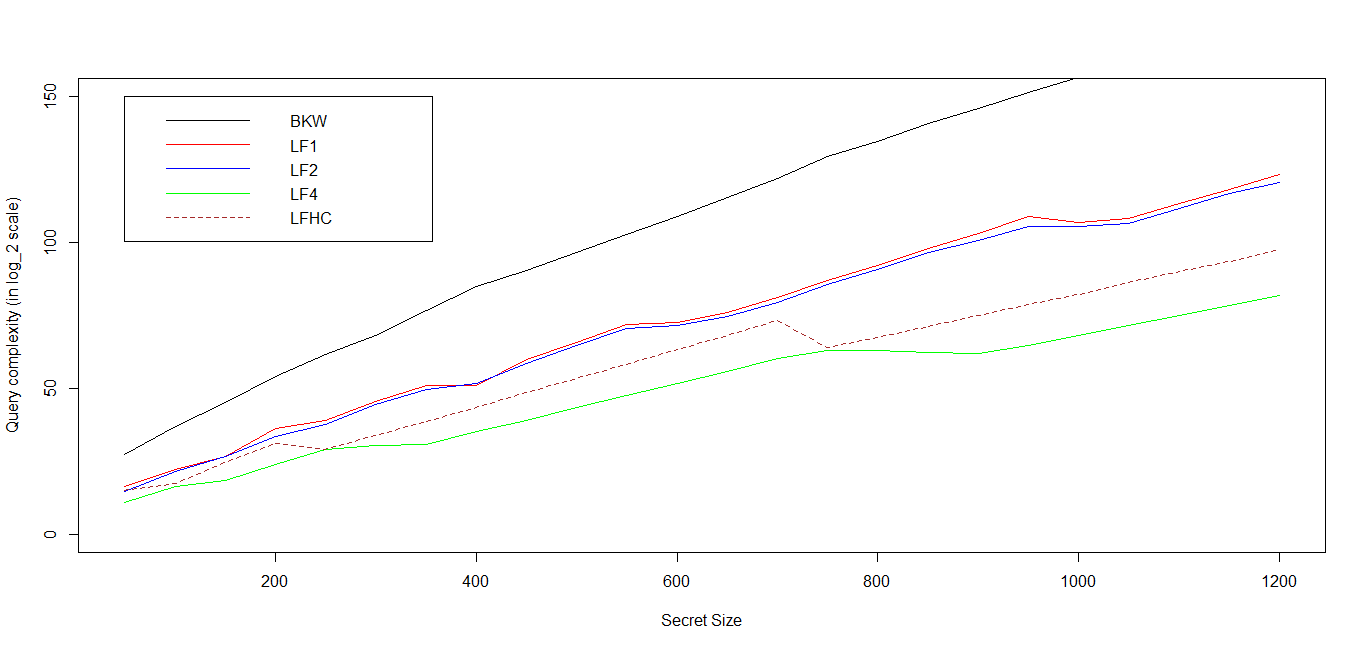
\includegraphics[width=\textwidth, height= 7.5cm]{LPNQuery}
 	 \caption{Query complexity ($\log_2q$) of Algorithms for $LPN_{s,n,\frac{1}{\sqrt{n}}}$ instance}
 	 \label{graph1}
 \end{figure}

 \begin{figure}
 	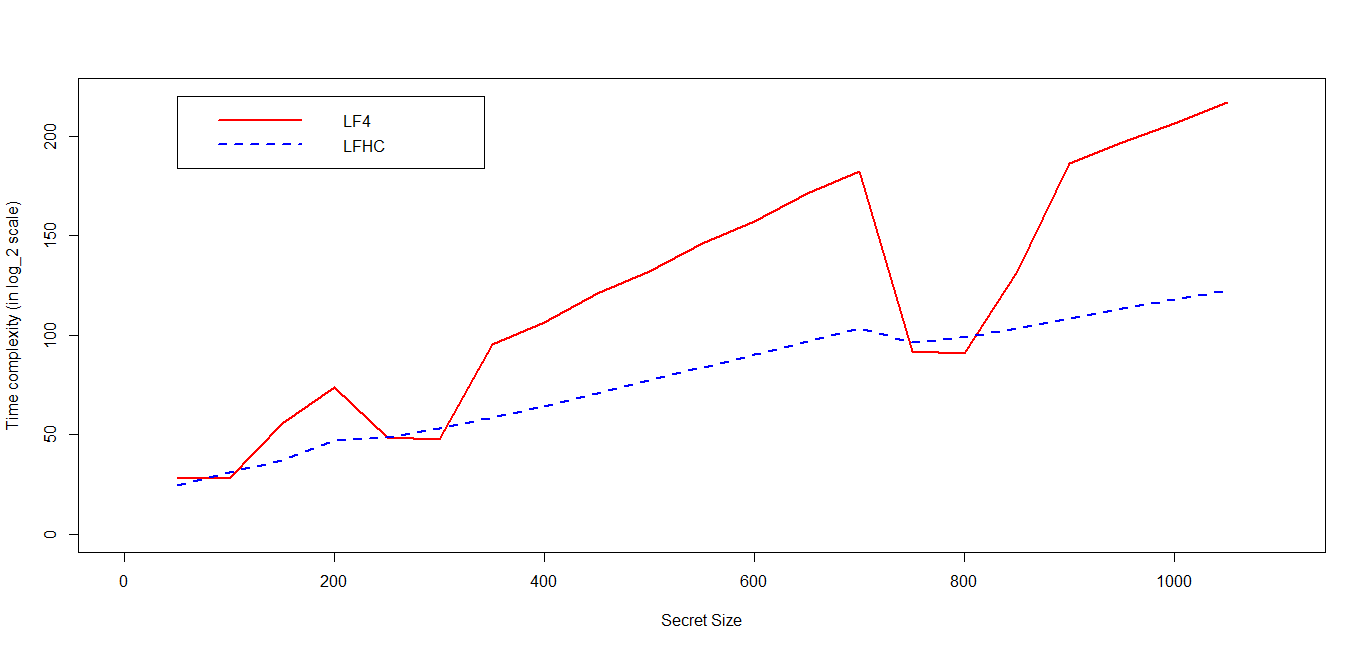
\includegraphics[width=\textwidth, height= 7.5cm]{LPNTime}
 	\caption{Time complexity ($\log_2t$) comparison of LF4 and LFHC at minimum query complexity for $LPN_{s,n,\frac{1}{\sqrt{n}}}$ instance}
 	\label{graph2}
 \end{figure}

 
 In figure \ref{graph1}, LF-HC's parameter $k$ is taken to be $4$ i.e. the reudction phase is same as LF4. We see that LF-HC has query complexity less than LF2, but more than LF4. However, it works close to LF4 in certain instances. In figure \ref{graph2}, the time complexities of LF4 and LFHC is shown when both of them acheives respective minimum query complexity. This shows with the cost of increasing query complexity a little bit, LFHC can outperform LF4 in terms of time complexity. However, for some specifics instances, where LF4 has lower time complexity than LFHC, it is the same instances where LFHC attains same query complexity as LF4. This occurs due to the fact that LFHC generally uses the reduction phase to reduce the size of secret to very fewer bits (usually less than 50) compared to the whole instance size  i.e. $n'=(n-ab)\leq50$. Compared to this, LF4 tends to have bigger block size $b$ and lower $a$ such that $n=ab$, hence one has to use the reduction phase $(a-1)$ times and the reduced secret size becomes of length $b=n-(a-1)b$ or close to $b$. Hence, implentation of Fast Walsh Hadamard transformation would yield a time complexity of $b2^b$ which is much bigger compared to the other terms existing in the time complexity of LF4. For certain instances, where LF4 and LFHC has same query complexity, LF4 reduces the secret to fewer bits like LFHC, hence $n'$ would be much lower than block size $b$. Therefore, in those instances, time complexity of LF4 would contain $n'2^{n'}$ which is much lesser than the other terms. This will ensure that it takes lesser time in those certain instances.
 
 \section{Conclusion}
 In this paper, I have tried to analyze how a generalized version of Levieil Fouque algorithm works and to what extend it can give a better result. The reduction phase of LF(k) uses an algorithm to solve Generalized Birthday Problem. Hence, the complexity of LF(k) can be greatly improved once the lower bound $2^{n'/k}$ is achieved in the Birthday Problem. Also, I have presented an algorithm based on Levieil Fouque generalized reduction, and using local decoding method of Hadamard code for solution phase. It can easily be understood that LF-HC which uses reduction of LF(k), performs better than LF(r) $\forall r<k$, and at the best, it may perform like LF(k) in terms of query complexity. Hence, we may call LF-HC as a bridge between BKW and LF algorithms. However, LF(k) algorithms sometimes fail to acheive smaller time complexity when it attends minimal query complexity, as seen in case with $LPN_{s,768,0.05}$ instance. In this sense, LF-HC uses the exact parameter to come up with optimal complexity faster, where the query complexity may increase a bit, but one can significantly reduce time and memory complexity. In practical scenario, one can precompute the complexities of LF(k) and LF-HC beforehand using the Complexity Theorems mentioned above and apply them in practical problems according to their preferences. 
 
 \section{Acknowledgements}
 I would like to express my sincere thanks to Dr. Goutam Paul of Indian Statistical Institute who had introduced this topic to me and gave me a golden opportunity to work on this as a part of my summer project under his supervision. 
 
  \begin{thebibliography}{99}
  	\bibitem{BKW} Avrim Blum, Adam Kalai and Hal Wasserman, 2003 --- \emph{Noise-tolerant Learning, the Parity problem and the Statistical Query Model}, ACM Press.\\
  	\bibitem{LF} Levieil É., Fouque PA. (2006) \emph{An Improved LPN Algorithm}. In: De Prisco R., Yung M. (eds) Security and Cryptography for Networks. SCN 2006. Lecture Notes in Computer Science, vol 4116. Springer, Berlin, Heidelberg\\
  	\bibitem{LFk} Bin Zhang, Lin Jiao and Mingsheng Wang, (2016) \emph{Faster Algorithms for Solving LPN} IACR-EUROCRYPT-2016, Cryptology ePrint Archive: Report 2016/275\\
  	\bibitem{LPNjournal} Sonia Bogos, Florian Tramer and Serge Vaudenay (2015), \emph{On Solving LPN using BKW and variants: Implementation and Analysis}, IACR Cryptology ePrint Archive:Report 2015/049\\
  	\bibitem{Ksum} David Wagner, 2002, \emph{A generalized Birthday Problem} --- In M.Yung, editor, \emph{Advances in Cryptology--CRYPTO 2002}, volume 2442 of \emph{Lecture Notes in Computer science}, pages 288-304, Springer Berlin Heidelberg, 2002.
  	\bibitem{hoeffding} Hoeffding W. :\emph{Probablity Inequalities for sums of Bounded Random Variable}, Journal of the American Statistical Association 58(301), 13-30 (1963).
  	 \\
  	
  \end{thebibliography}
\end{document}